\chapter{Methodik}
\label{chap:methodik}

In diesem Kapitel wird der methodische Aufbau dieser Thesis beschrieben und begründet.
Die Arbeit ist als industrielle Fallstudie in Zusammenarbeit mit \emph{levigo solutions} konzipiert und dient der Evaluation des \gls{mmf} an einer bestehenden Microservices-Architektur.
Diese Fallstudie besteht aus zwei Hauptbestandteilen.
Im ersten Teil wird ein Refactoring des Produktes \emph{jadice flow} nach Anleitung des Frameworks durchgeführt.
Im zweiten Teil wird das Ergebnis dieses Refactorings verwendet, um eine Evaluation des Frameworks und Werkzeugs abzuschließen.

\section{Refactoring mit \gls{mmf}}

Die Vorgehensweise beim Refactoring ist durch das Framework sehr genau vorgegeben, daher wird das Refactoring in dieser Thesis in die gleichen drei Phasen unterteilt wie in \cref{sec:mmf} beschrieben.
In der ersten Phase wird ein Architekturreview nach \Citet{SVAHNBERG20071893} mit den Stakeholdern des Produkts durchgeführt.
Diese Methode wird in \cref{sec:methodik-architekturreview} näher beschrieben.
Das wesentliche Ergebnis dieses Reviews sind die gewünschten \glspl{qa} des Systems.
Diese Attribute sind die Basis für Phase 2 und 3 und werden in den \gls{arh} eingegeben.
Dieser führt Berechnungen mit den \glspl{qa} durch und kann so eine Liste von Refactoring-Methoden vorschlagen, die nach ihrer Eignung für die \glspl{qa} sortiert sind.
Als weitere Eingabe dafür dienen bestimmte Filter, die in \cref{sec:durchführung-phase2} näher erläutert werden.
Aus der resultierenden Liste von Migrationsmethoden werden die besten Vorschläge betrachtet und bewertet, bevor einer davon ausgewählt und in den folgenden Phasen verwendet wird.
Analog dazu wird in Phase 3a eine sortierte Liste von Patterns und Best Practices vorgeschlagen, ebenfalls durch Eingabe von \glspl{qa} und Filtern.
Das Vorgehen bei der Auswahl der Filter sowie die spätere Inspektion der Vorschläge des \gls{arh} werden in Form von strukturierten Feldnotizen protokolliert.
Deren genauere Funktion und Form dieser wird folgend in \cref{sec:structured-field-notes} erläutert.

\subsection{Architekturreview}
\label{sec:methodik-architekturreview}

Das Architekturreview nach \Citet{SVAHNBERG20071893} basiert auf Szenarien-basierten Methoden, wie der \gls{saam} (\Citet{saam}) und der \gls{atam} (\Citet{kazman_2000}).
Das bedeutet, dass die gewünschten \glspl{qa} des Systems in Form von Szenarien erfasst und dokumentiert werden.
Dabei werden mit jedem Szenario zugehörige \glspl{qa} assoziiert, wodurch am Ende eine Abbildung aller \glspl{qa} auf ihre Priorität möglich ist.
Diese Abbildung ist das eigentliche Ergebnis, das der \gls{arh} als Eingabe für die weiteren Phasen benötigt.
Die Szenarien sind dabei lediglich ein Zwischenprodukt und sollen dabei helfen, eine genauere Vorstellung davon zu bekommen, welche spezifischen Situationen mit den \glspl{qa} verbunden sind.
Sie ermöglichen auch eine Bewertung der Wichtigkeit und technischen Schwierigkeit anhand konkreter Situationen, was bei abstrakten \glspl{qa} schwieriger wäre.

Um die wichtigsten Szenarien und \glspl{qa} zu ermitteln, haben \Citet{SVAHNBERG20071893} einen sechsschrittigen Plan entwickelt.
Diese sollen in einer etwa vierstündigen moderierten Gruppendiskussion mit den wichtigsten Stakeholdern des Produkts durchgeführt werden.
Im ersten Schritt gibt der \gls{po} eine Einführung in das Projekt, in der Ziele für das Produkt sowie die Organisation geschildert werden.
Danach beginnt im Schritt 2 die Identifikation der \glspl{qa} in einer Brainstorming-Runde mit Beteiligung von \gls{po}, End-Nutzer und Architekten.
Die Liste der Qualitätskriterien gemäß ISO 9126~\cite{ISO-9126}\cite{ISO-9126-b} dient dabei als Vorlage für mögliche \glspl{qa}.
Im dritten Schritt ordnen \gls{po} und End-Nutzer die Liste der \glspl{qa} nach Wichtigkeit und fügen den drei wichtigsten jeweils zwei Szenarien hinzu.
Nach einer Pause präsentiert im vierten Schritt ein Softwarearchitekt die vorgeschlagene Architektur.
Anschließen werden im fünften Schritt die Szenarien nacheinander durchgegangen, analysiert und bewertet, inwiefern sie durch die Architektur erfüllt werden und wo etwaige Probleme bestehen.
Im sechsten Schritt werden alle festgestellten Probleme und Aspekte, die mehr Aufmerksamkeit benötigen, final diskutiert und der gesamte Prozess wird zusammengefasst.

Entgegen der eigentlichen Zielsetzung der Bewertung des Systems durch das Architekturreview nach \Citet{SVAHNBERG20071893} ist das Ziel des Reviews in dieser Thesis ein anderes.
Das gewünschte Ergebnis sind in diesem Fall lediglich die \glspl{qa} in Form von Szenarien, die in mit dem \gls{arh} verwendet werden können.
Die Schritte 4,5 und 6 werden daher nicht durchgeführt, da diese hauptsächlich der Bewertung des Systems unter den definierten \glspl{qa} dienen sollen.
Außerdem entfällt Schritt 1, da alle Teilnehmer des Architekturreviews bestens mit dem Produkt vertraut sind und schon einige Zeit daran arbeiten.
Somit bleiben im Wesentlichen nur noch Schritt 2 und 3 für diesen Anwendungsfall übrig.
Diese wurden zusätzlich noch weiter auf die Verwendung mit dem \gls{arh} angepasst.
Im Schritt 2 werden als Basis-\glspl{qa} statt der ISO 9126~\cite{ISO-9126} die von \Citet{master-daniel-koch} speziell für Microservices-Architekturen identifizierten \glspl{qa} (siehe \cref{fig:qas}) verwendet.
Dabei handelt es sich zu großen Teilen um die nach der Literaturrecherche wichtigsten \glspl{qa} aus der ISO 25010~\cite{ISO-25010}, die durch wenige Microservices-spezifische \glspl{qa} ergänzt wurden.
\begin{figure}
	\centering
	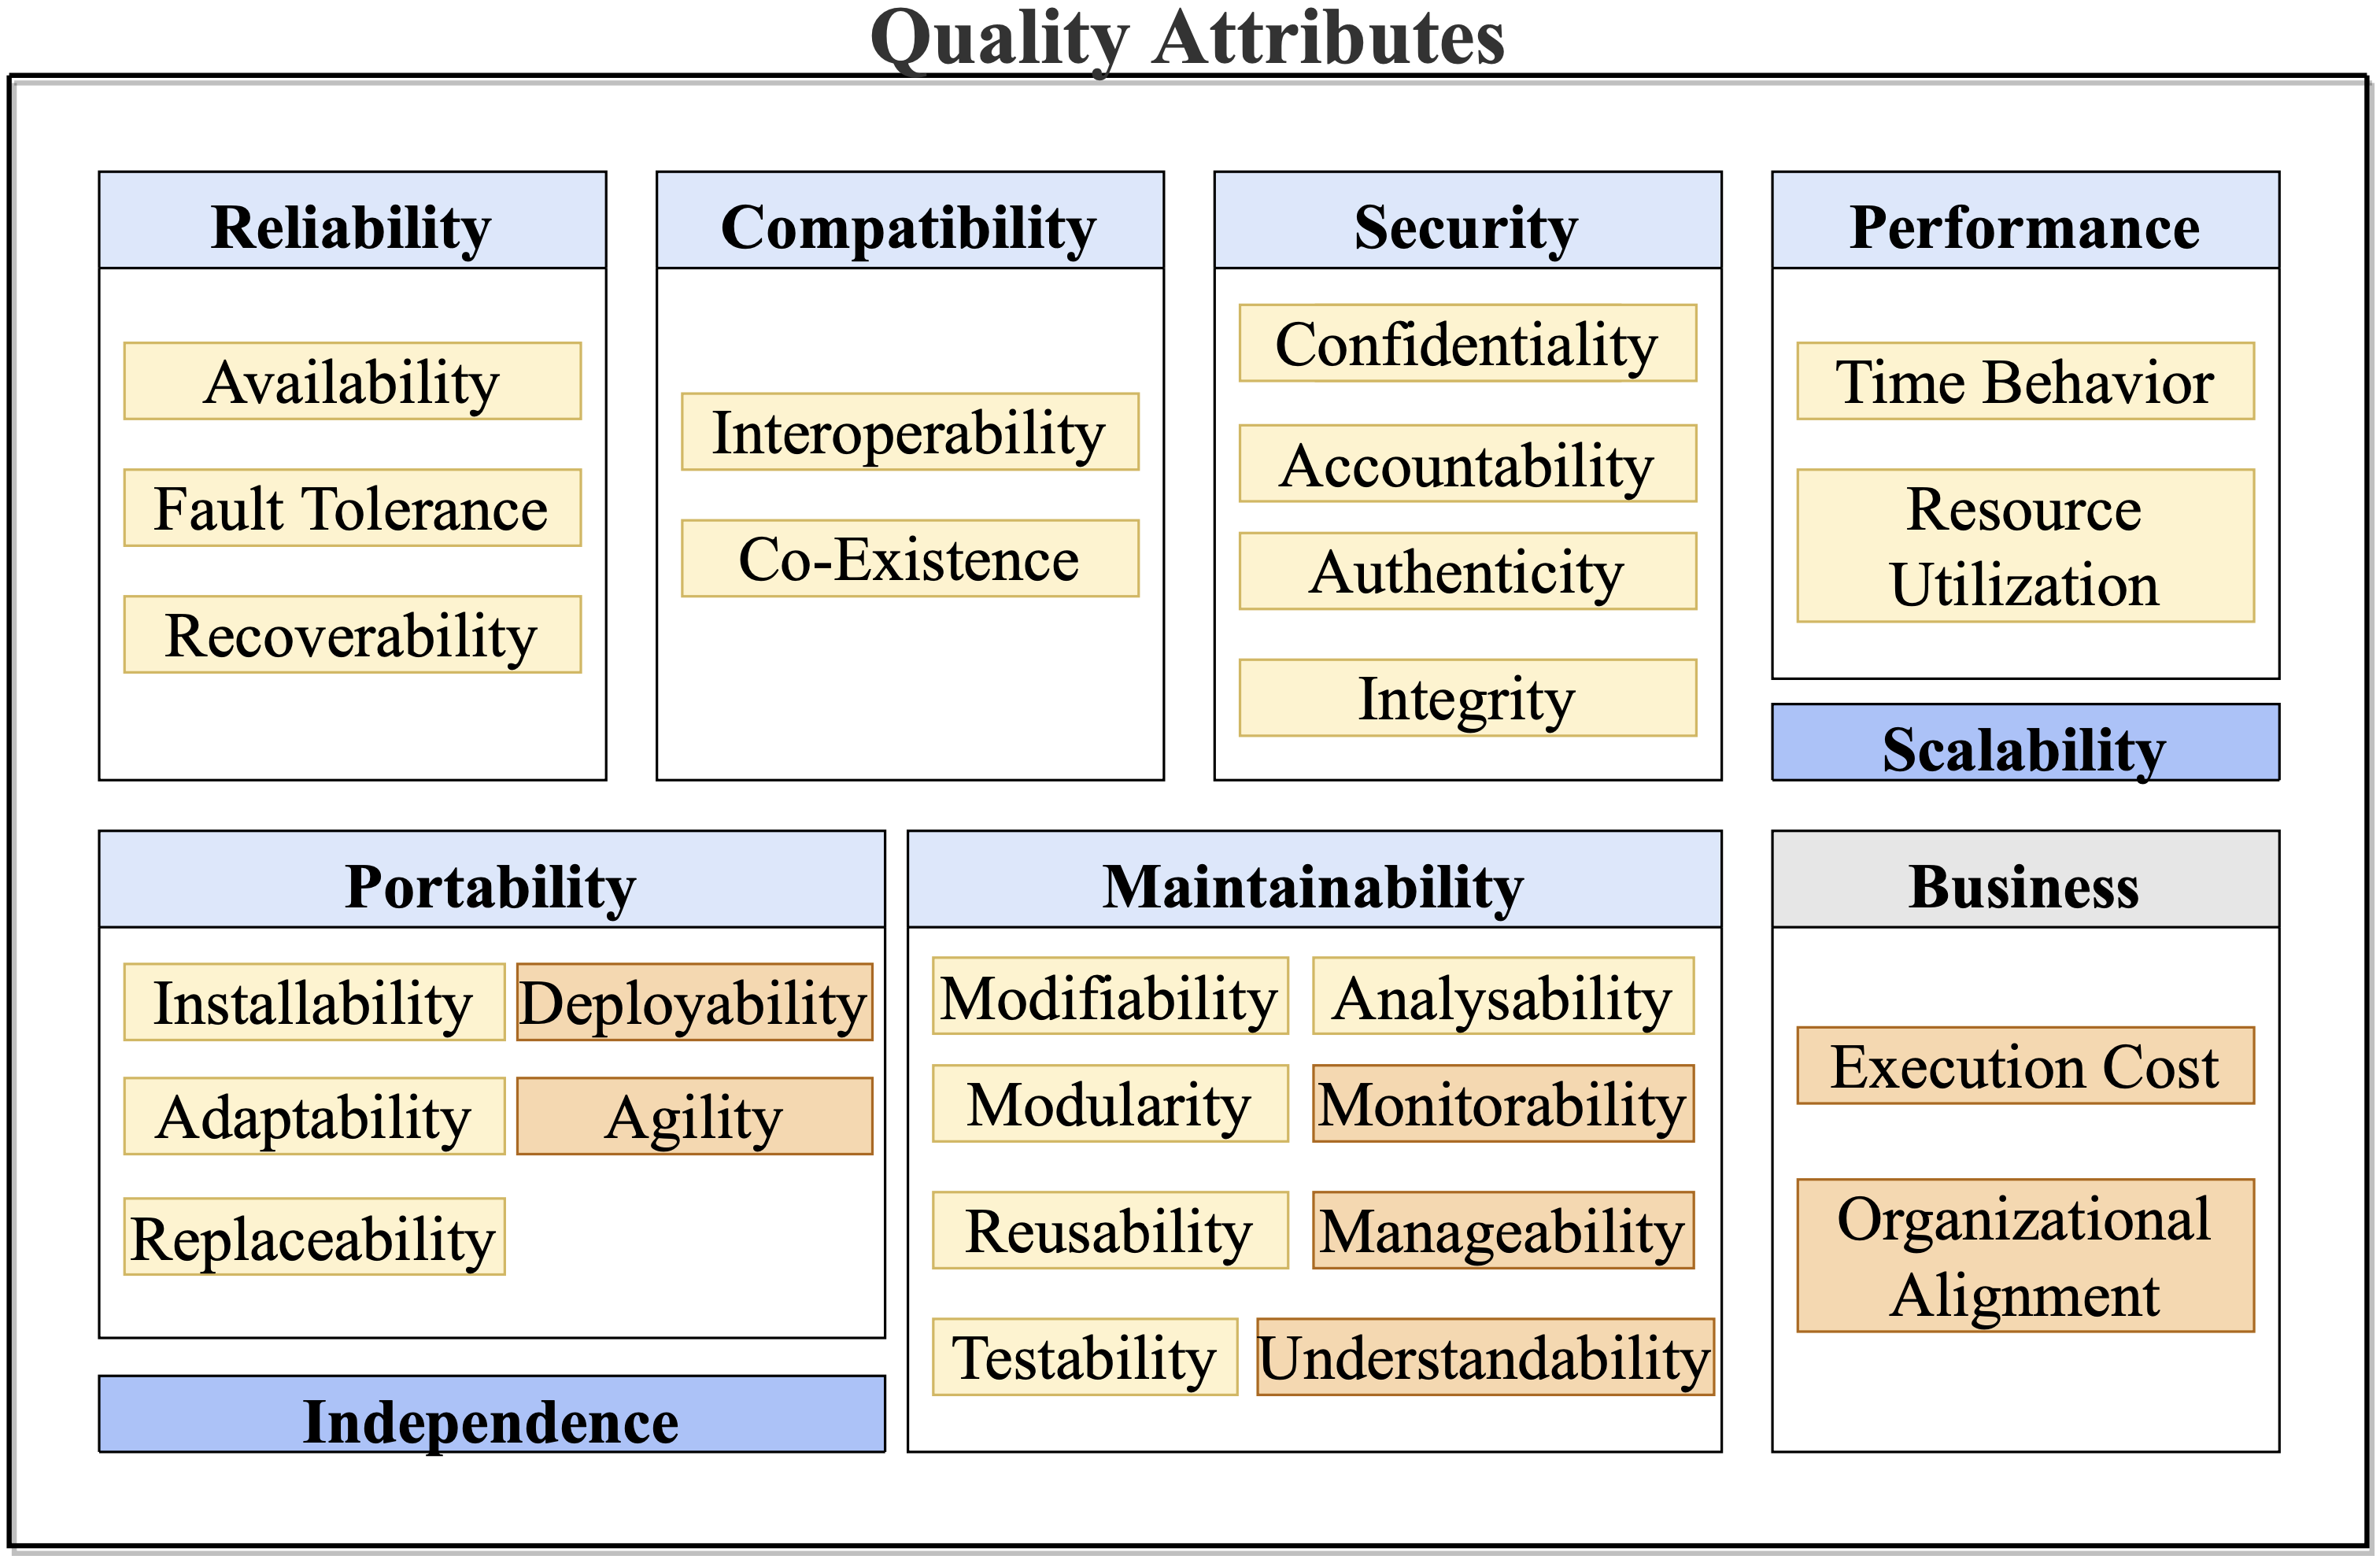
\includegraphics[width=\textwidth]{qas}
	\caption[Spezielle \acrlongpl{qa} für Microservices-Architekturen]{
		Spezielle \acrfullpl{qa} für Microservices-Architekturen nach \Citet{master-daniel-koch}.
	}
	\label{fig:qas}
\end{figure}
Abgesehen davon, dass diese besser an die Architektur angepasst sind, ist es notwendig, diese zu verwenden, da der \gls{arh} nur diese zur Auswahl hat.
In der Vorlage von \Citet{SVAHNBERG20071893} war zwar keine vergleichbare explizite Bewertung oder Priorisierung der Szenarien gegeben.
Das ist allerdings aufgrund des Kontexts durch die qualitative Bewertung durch Menschen nicht nötig.
Im Vergleich dazu können bei der automatisierten Auswertung durch ein Werkzeug wie den \gls{arh} die Szenarien nicht automatisch eingeschätzt werden.
Aus diesem Grund erfolgt in Schritt 3 zusätzlich eine dreistufige Bewertung der Szenarien hinsichtlich ihrer Wichtigkeit und technische Schwierigkeit.
Die Bewertung erfolgt von A-C bewertet, wobei A für sehr wichtig und sehr technisch schwierig steht.

\subsection{Strukturierte Feldnotizen}
\label{sec:structured-field-notes}

Während Phase 1 also in einer Fokusgruppe durchgeführt wurde, findet die Bearbeitung in den folgenden Phasen größtenteils in Einzelarbeit statt.
Um dabei strukturiert zu protokollieren, welche Aktivitäten im Rahmen dieser Phasen durchgeführt wurden, werden systematisch durchgeführte Aktivitäten mit gemachten Erfahrungen und Herausforderungen dokumentiert und am Ende ausgewertet.
Dazu werden strukturierte Feldnotizen verwendet~\cite{seaman2008qualitative}.
Dabei können die involvierten Stakeholder zur Rate gezogen werden.


\section{Evaluation des \gls{mmf}}

Das bis inklusive Phase 3a geplante Refactoring soll dann in Phase 3b im Rahmen eines minimalen Prototyps umgesetzt und simuliert werden, da ein Refactoring des kompletten Systems im zeitlichen Rahmen dieser Arbeit nicht möglich wäre.
Dabei entstehende Prototypen könnten Vorläufer von \emph{jadice flow 2.0} werden.

Im Nachgang sollen die Ergebnisse dieses Experiments ausgewertet werden. Um quantitativ vergleichbare Ergebnisse zu erhalten, sollen im Vorlauf des Experiments Vergleichskriterien und Messmethoden definiert werden, die es möglich machen, gleichartige Anwendungsfälle von \emph{jadice flow 1.0} und neuen Prototypen zu vergleichen.
